\section{Fourier Transform}
\label{sec:fourier transform}

\subsection{Objective}
We plot a Rectangular Pulse Signal $x(t)$ in \textit{Matlab} and explore 
its magnitude and phase spectrum of its Fourier Transform.

\subsection{Theory}

MATLAB is a programming language and environment that is widely used for
scientific computing, numerical analysis, and data visualization. It is designed to
support matrix and vector operations, which are fundamental to many scientific and
engineering applications.

The Fourier Transform of a signal $x(t)$ is defined as
\begin{equation}
	X(\omega) = \int_{-\infty}^{\infty} x(t) e^{-j\omega t} dt
\end{equation}

The Fourier Transform of a rectangular pulse is given by
\begin{equation}
	X(\omega) = \frac{1}{2\pi} \int_{-\infty}^{\infty} \frac{1}{\sqrt{1 - (\omega t)^2}} dt
\end{equation}

The magnitude and phase spectrum of the Fourier Transform of a rectangular pulse is given by
\begin{equation}
	|X(\omega)| = \frac{1}{\pi} \sqrt{\frac{\pi}{2} - \omega^2}
\end{equation}
\begin{equation}
	\angle X(\omega) = \frac{\pi}{2} - \arctan(\omega)
\end{equation}


\subsection{Matlab Code}

\inputminted[fontsize=\footnotesize,autogobble]{matlab}{code/fourier.m}

\subsection{Output}

\begin{figure}[!htb]
	\centering
	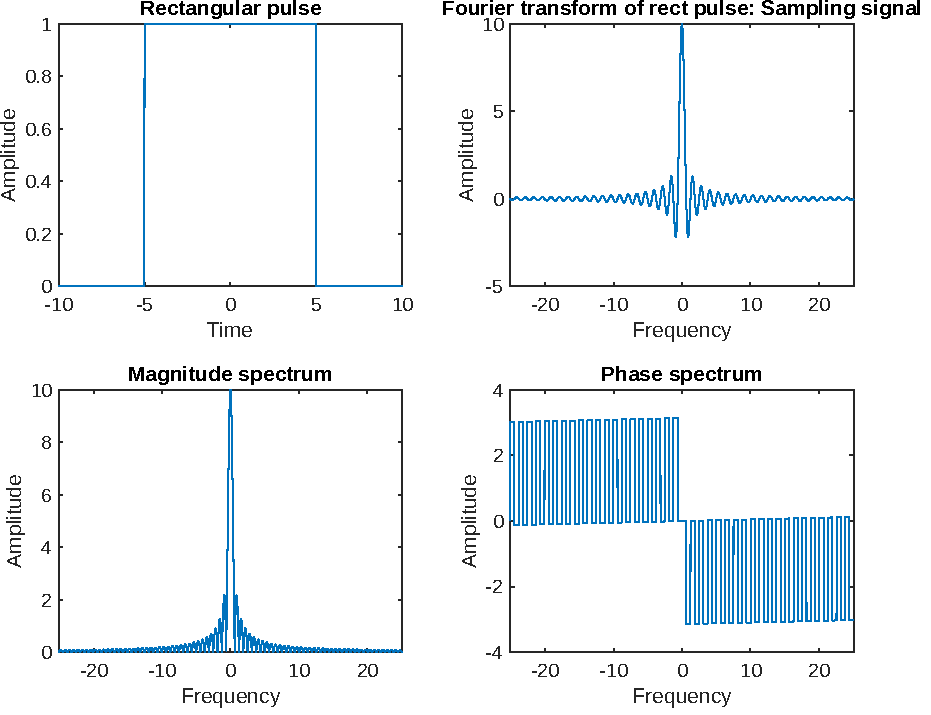
\includegraphics[width=0.7\textwidth]{res/figures/Figure_1.pdf}
	\label{output:fourier transform}
	\caption{Fourier Transform}
\end{figure}